% begin module tangent-line-polynomial
\begin{frame}
\begin{example}[Tangent line to a polynomial]
Find an equation for the tangent line to the parabola $y = x^2 +2x + 1$ at the point $P = (2,9)$.

\begin{columns}[c]
\column{.4\textwidth}
\psset{xunit=0.5cm, yunit=0.5cm}
\begin{pspicture}(-5, -5)(5,5) 
\psframe*[linecolor=white](-5,-5)(5,15) 
\tiny
\psaxes{->}(0,0)(-3.2,-0.5)(3.2,12)
%Function formula: 1+2 (x)+(x)^{2} 
\uncover<8->{
\psline[linecolor=blue](0.416666667,-0.5)(2.5,12)
}
\psplot[linecolor=red, plotpoints=1000]{-2.6}{2.4}{x 2 exp x 2 mul add 1 add }
\psFullDotBlack{2}{9}
\rput(-3, 5) {\tiny$y=x^2+2x+1$}
\end{pspicture} 
%\only<-7>{%
%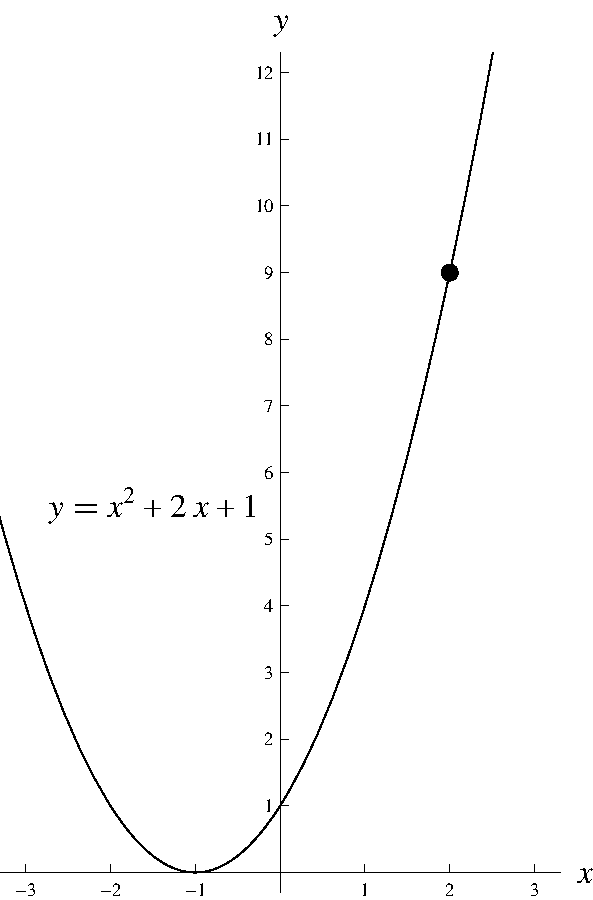
\includegraphics[width=4.0cm]{derivatives/pictures/tangent-line-polynomiala.pdf}%
%}%
%\only<8->{%
%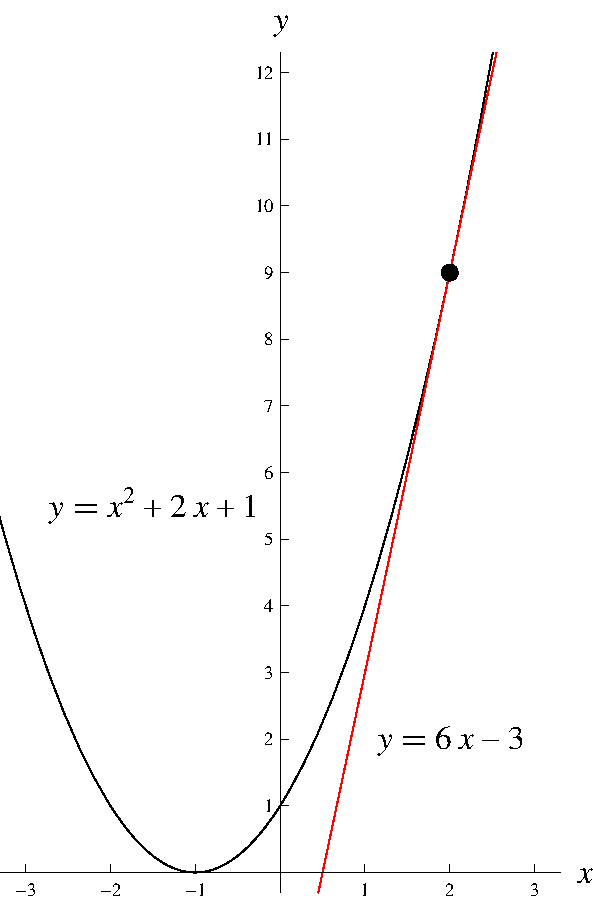
\includegraphics[width=4.0cm]{derivatives/pictures/tangent-line-polynomialb.pdf}%
%}%
\column{.6\textwidth}
\uncover<2->{%
Here \alert<handout:0| 2-3>{$a = \uncover<3->{2}$} and $f(x) = x^2 + 2x +1$.
}%
\abovedisplayskip=0pt
\belowdisplayskip=0pt
\abovedisplayshortskip=0pt
\belowdisplayshortskip=0pt
\begin{align*}
\uncover<3->{m} & \uncover<3->{ = }  %
\uncover<3->{\lim_{x\rightarrow 2} \frac{f(x)-f(2)}{x-2}}\\
& \uncover<4->{ = }  %
\uncover<4->{\lim_{x\rightarrow 2}\frac{(x^2+ 2 x +1) - 9}{x-2} }\\
& \uncover<5->{ = }  %
\uncover<5->{\lim_{x\rightarrow 2}\frac{x^2+ 2 x - 8}{x-2}}\\
& \uncover<6->{ = }  %
\uncover<6->{\lim_{x\rightarrow 2}\frac{(x - 2)(x+4)}{x-2}}\\
& \uncover<7->{ = }  %
\uncover<7->{\lim_{x\rightarrow 2} (x+4)} \uncover<8>{= 6.}\\
\end{align*}
\uncover<8->{
The tangent line: $y = 6x - 3$.
}
\end{columns}
\end{example}
\end{frame}
% end module tangent-line-polynomial
